% 八个数据集名与八幅原图不变；只替换下方自然语言描述。
\begin{tikzpicture}
\node[anchor=south west,inner sep=0] (im) at (0,0) {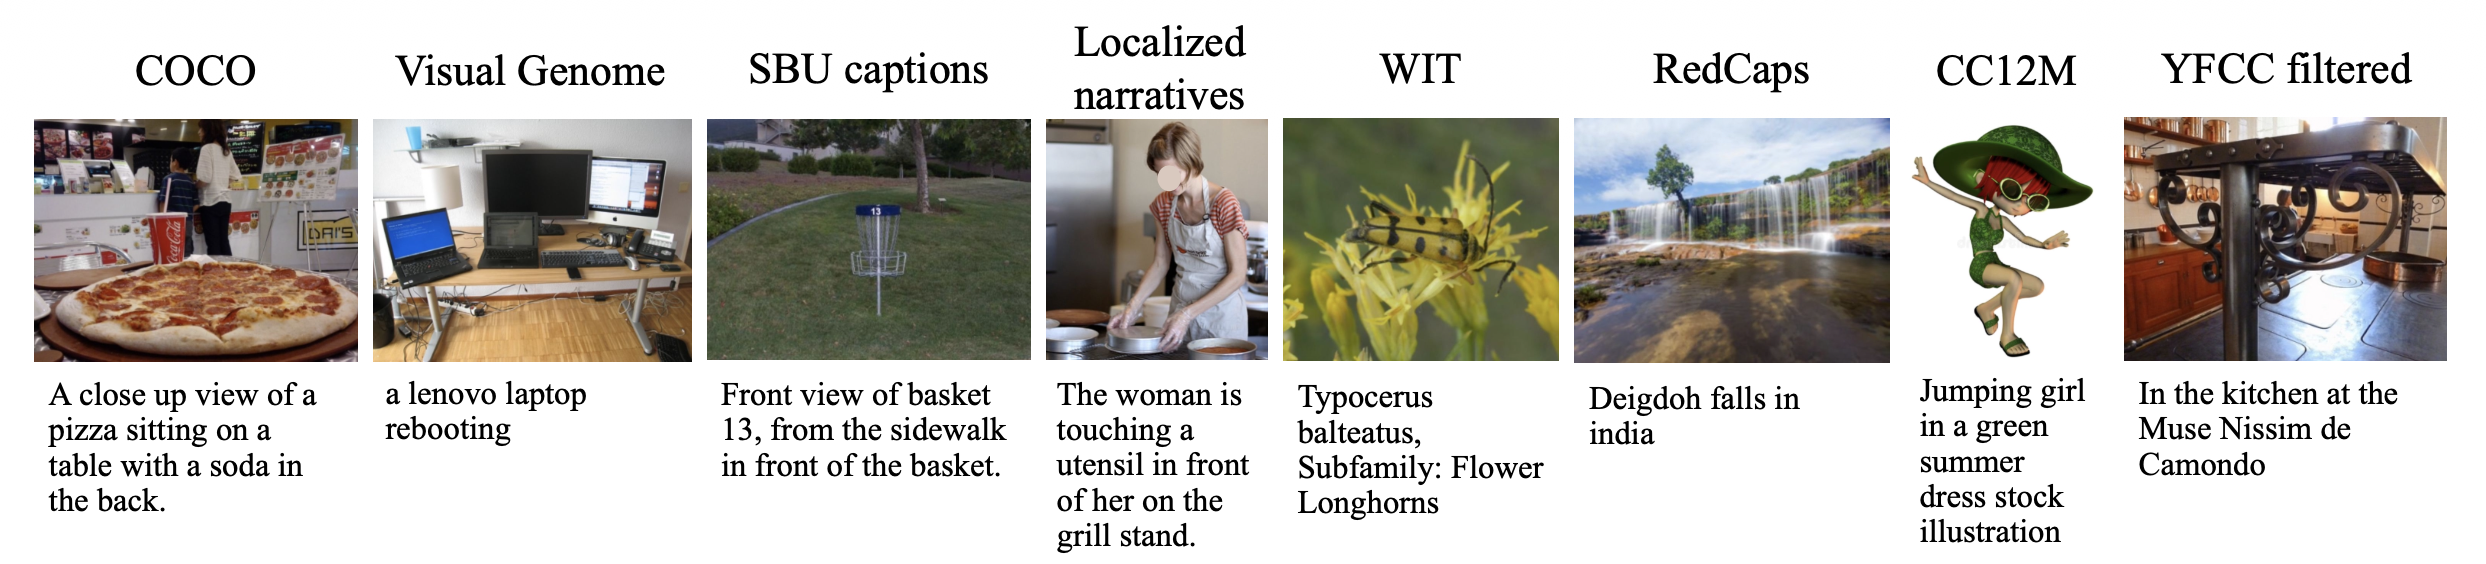
\includegraphics[width=\linewidth]{figures/flava.png}};
\begin{scope}[x={(im.south east)},y={(im.north west)}]
\fill[white] (0,0) rectangle (1,.337);
\node[anchor=north west,align=left,inner sep=0pt,text width=.113\linewidth,font=\fontsize{7}{8.5}\selectfont] at (.013,.323) {桌上一份披萨的特写，后方放着一杯汽水。};
\node[anchor=north west,align=left,inner sep=0pt,text width=.113\linewidth,font=\fontsize{7}{8.5}\selectfont] at (.154,.323) {一台正在重新启动的 Lenovo 笔记本电脑。};
\node[anchor=north west,align=left,inner sep=0pt,text width=.113\linewidth,font=\fontsize{7}{8.5}\selectfont] at (.291,.323) {从篮筐前的人行道正面看 13 号篮筐。};
\node[anchor=north west,align=left,inner sep=0pt,text width=.087\linewidth,font=\fontsize{7}{8.5}\selectfont] at (.425,.323) {女子正在触碰她面前烤架上的一件器具。};
\node[anchor=north west,align=left,inner sep=0pt,text width=.103\linewidth,font=\fontsize{7}{8.5}\selectfont] at (.523,.323) {\textit{Typocerus balteatus}，亚科：花天牛。};
\node[anchor=north west,align=left,inner sep=0pt,text width=.113\linewidth,font=\fontsize{7}{8.5}\selectfont] at (.640,.323) {印度的 Deigdoh 瀑布。};
\node[anchor=north west,align=left,inner sep=0pt,text width=.078\linewidth,font=\fontsize{7}{8.5}\selectfont] at (.773,.323) {身穿绿色夏季连衣裙、跃起的女孩，素材插画。};
\node[anchor=north west,align=left,inner sep=0pt,text width=.122\linewidth,font=\fontsize{7}{8.5}\selectfont] at (.862,.323) {在 Muse Nissim de Camondo 博物馆的厨房中。};
\end{scope}
\end{tikzpicture}
